\documentclass[a4paper,10pt,twocolumn]{article}
%%%%%%%%%%%%%%%%%%%%%%%%%%%%%%%%%%%%%%%%%
% Wenneker Article
% Structure Specification File
% Version 1.0 (28/2/17)
%
% This file originates from:
% http://www.LaTeXTemplates.com
%
% Authors:
% Frits Wenneker
% Vel (vel@LaTeXTemplates.com)
%
% License:
% CC BY-NC-SA 3.0 (http://creativecommons.org/licenses/by-nc-sa/3.0/)
%
%%%%%%%%%%%%%%%%%%%%%%%%%%%%%%%%%%%%%%%%%

%----------------------------------------------------------------------------------------
%	PACKAGES AND OTHER DOCUMENT CONFIGURATIONS
%----------------------------------------------------------------------------------------

\usepackage[english]{babel} % English language hyphenation

\usepackage{microtype} % Better typography

\usepackage{amsmath,amsfonts,amsthm} % Math packages for equations

\usepackage[svgnames]{xcolor} % Enabling colors by their 'svgnames'

\usepackage[hang, small, labelfont=bf, up, textfont=it]{caption} % Custom captions under/above tables and figures

\usepackage{booktabs} % Horizontal rules in tables

\usepackage{lastpage} % Used to determine the number of pages in the document (for "Page X of Total")

\usepackage{graphicx} % Required for adding images

\usepackage{enumitem} % Required for customising lists
\setlist{noitemsep} % Remove spacing between bullet/numbered list elements

\usepackage{sectsty} % Enables custom section titles
\allsectionsfont{\usefont{OT1}{phv}{b}{n}} % Change the font of all section commands (Helvetica)

%----------------------------------------------------------------------------------------
%	MARGINS AND SPACING
%----------------------------------------------------------------------------------------

\usepackage{geometry} % Required for adjusting page dimensions

\geometry{
	top=1cm, % Top margin
	bottom=1.5cm, % Bottom margin
	left=2cm, % Left margin
	right=2cm, % Right margin
	includehead, % Include space for a header
	includefoot, % Include space for a footer
	%showframe, % Uncomment to show how the type block is set on the page
}

\setlength{\columnsep}{7mm} % Column separation width

%----------------------------------------------------------------------------------------
%	FONTS
%----------------------------------------------------------------------------------------

\usepackage[T1]{fontenc} % Output font encoding for international characters
\usepackage[utf8]{inputenc} % Required for inputting international characters

\usepackage{XCharter} % Use the XCharter font

%----------------------------------------------------------------------------------------
%	HEADERS AND FOOTERS
%----------------------------------------------------------------------------------------

\usepackage{fancyhdr} % Needed to define custom headers/footers
\pagestyle{fancy} % Enables the custom headers/footers

\renewcommand{\headrulewidth}{0.0pt} % No header rule
\renewcommand{\footrulewidth}{0.4pt} % Thin footer rule

\renewcommand{\sectionmark}[1]{\markboth{#1}{}} % Removes the section number from the header when \leftmark is used

%\nouppercase\leftmark % Add this to one of the lines below if you want a section title in the header/footer

% Headers
\lhead{} % Left header
\chead{\textit{\thetitle}} % Center header - currently printing the article title
\rhead{} % Right header

% Footers
\lfoot{} % Left footer
\cfoot{} % Center footer
\rfoot{\footnotesize Page \thepage\ of \pageref{LastPage}} % Right footer, "Page 1 of 2"

\fancypagestyle{firstpage}{ % Page style for the first page with the title
	\fancyhf{}
	\renewcommand{\footrulewidth}{0pt} % Suppress footer rule
}

%----------------------------------------------------------------------------------------
%	TITLE SECTION
%----------------------------------------------------------------------------------------

\newcommand{\authorstyle}[1]{{\large\usefont{OT1}{phv}{b}{n}\color{DarkRed}#1}} % Authors style (Helvetica)

\newcommand{\institution}[1]{{\footnotesize\usefont{OT1}{phv}{m}{sl}\color{Black}#1}} % Institutions style (Helvetica)

\usepackage{titling} % Allows custom title configuration

\newcommand{\HorRule}{\color{DarkGoldenrod}\rule{\linewidth}{1pt}} % Defines the gold horizontal rule around the title

\pretitle{
	\vspace{-30pt} % Move the entire title section up
	\HorRule\vspace{10pt} % Horizontal rule before the title
	\fontsize{32}{36}\usefont{OT1}{phv}{b}{n}\selectfont % Helvetica
	\color{DarkRed} % Text colour for the title and author(s)
}

\posttitle{\par\vskip 15pt} % Whitespace under the title

\preauthor{} % Anything that will appear before \author is printed

\postauthor{ % Anything that will appear after \author is printed
	\vspace{10pt} % Space before the rule
	\par\HorRule % Horizontal rule after the title
	\vspace{20pt} % Space after the title section
}

%----------------------------------------------------------------------------------------
%	ABSTRACT
%----------------------------------------------------------------------------------------

\usepackage{lettrine} % Package to accentuate the first letter of the text (lettrine)
\usepackage{fix-cm}	% Fixes the height of the lettrine

\newcommand{\initial}[1]{ % Defines the command and style for the lettrine
	\lettrine[lines=3,findent=4pt,nindent=0pt]{% Lettrine takes up 3 lines, the text to the right of it is indented 4pt and further indenting of lines 2+ is stopped
		\color{DarkGoldenrod}% Lettrine colour
		{#1}% The letter
	}{}%
}

\usepackage{xstring} % Required for string manipulation

\newcommand{\lettrineabstract}[1]{
	\StrLeft{#1}{1}[\firstletter] % Capture the first letter of the abstract for the lettrine
	\initial{\firstletter}\textbf{\StrGobbleLeft{#1}{1}} % Print the abstract with the first letter as a lettrine and the rest in bold
}

%----------------------------------------------------------------------------------------
%	BIBLIOGRAPHY
%----------------------------------------------------------------------------------------

\usepackage[backend=bibtex,style=authoryear,natbib=true]{biblatex} % Use the bibtex backend with the authoryear citation style (which resembles APA)

\addbibresource{example.bib} % The filename of the bibliography

\usepackage[autostyle=true]{csquotes} % Required to generate language-dependent quotes in the bibliography

\usepackage{subfigure}
\title{Subsitution of AraR operon}
\date{\today}
\begin{document}
    \thispagestyle{firstpage}
    \maketitle
    \lettrineabstract{Since weeks have we stuck in the search of the mathematical model of AraR and AraE promoter in Bacillus $subtilis$,
    but apparently, no progress has been made because a minor field it is to research arabinose operon in Bacillus $subtilis$.
    Hence we need to come up with a alternative choice:subsitute the AraR with a negative regulatory operon in E.$coli$.}
    \section{Similarity of LacI and AraR}
    As we have learnt in molecular biology,LacI promotion sysytem is a negative regulation sysytem.As the concentration of lactose rises ,LacI will binds to 
    arabinose and then release from $lacI$,relieve the cell form the negative regulation.People call this status \textbf{induced} state.\citep{Kuhlman2007}

    Lac is not a mono protein,it is a protein in consists of two asymmetric subunits,which will be transcripted and translated in dependent of lacZY,which are the 
    structural gene of lactose operon.The presence of lactose will change the formation of two LacI subunits,which lead to a loss of interaction between protein 
    and DNA.Such a contraption will enable LacI to response to the change of lactose level.
    \begin{figure}
        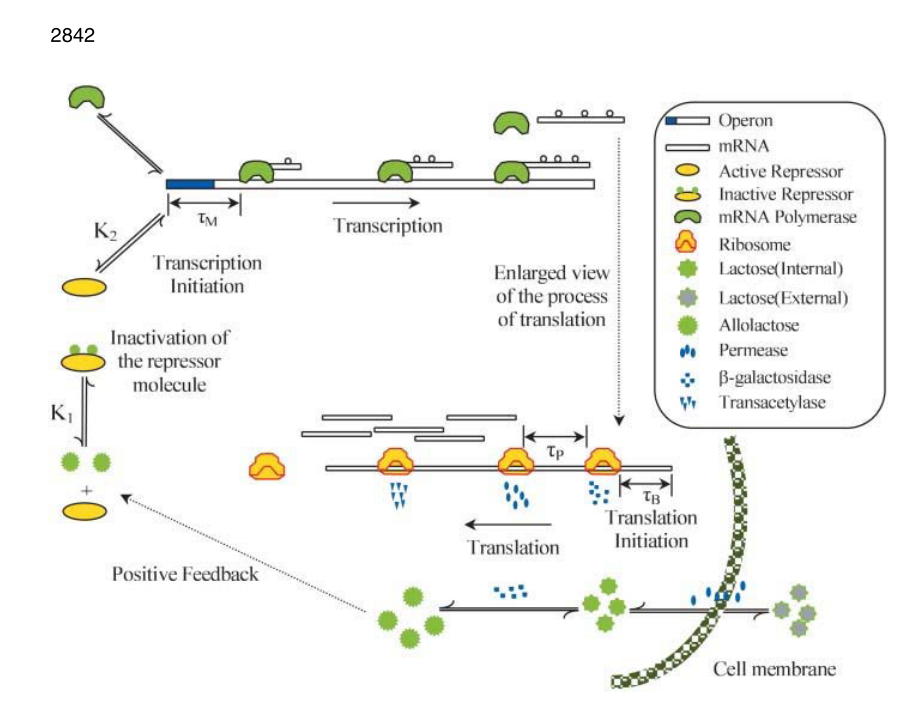
\includegraphics[width=\linewidth]{Picture/lac.png} % Figure image
        \caption{Summary of Lac operon} % Figure caption
        \label{lac} % Label for referencing with \ref{bear}
    \end{figure}
    
    It's also discovered that AraR in $Bacillus subtilis$ functions in a same pattern as LacI ,it is also a nagetive regulatory operon.The raise of arabinose
    concentration will lead to the release of AraR from promoter AraE.The mechanism of AraR to regulate the expression is very close to what will happend on LacI.
    \begin{figure}
        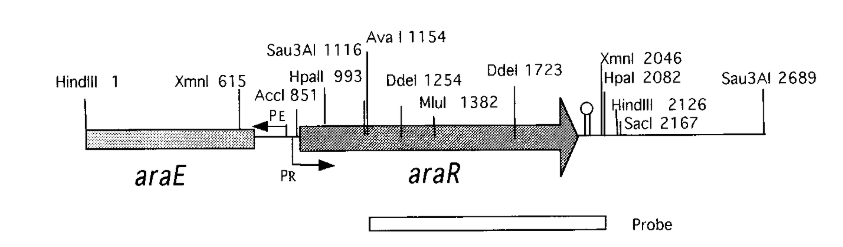
\includegraphics[width=\linewidth]{Picture/ara.png} % Figure image
        \caption{Summary of Ara operon} % Figure caption
        \label{ara} % Label for referencing with \ref{bear}
    \end{figure}

    Apart from theoretic summary,these two operon also present many similarity in experimental data.Taking the expression data into consideration \ref{compare}
    \begin{figure}
        \subfigure[ara]{
            \begin{minipage}[t]{0.5\linewidth}
            \centering
            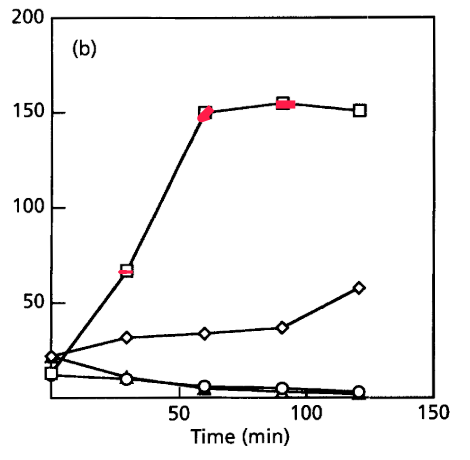
\includegraphics[width=1in]{Picture/ara-induced.png}
            %\caption{fig1}
            \end{minipage}%
            }%
            \subfigure[lac]{
            \begin{minipage}[t]{0.5\linewidth}
            \centering
            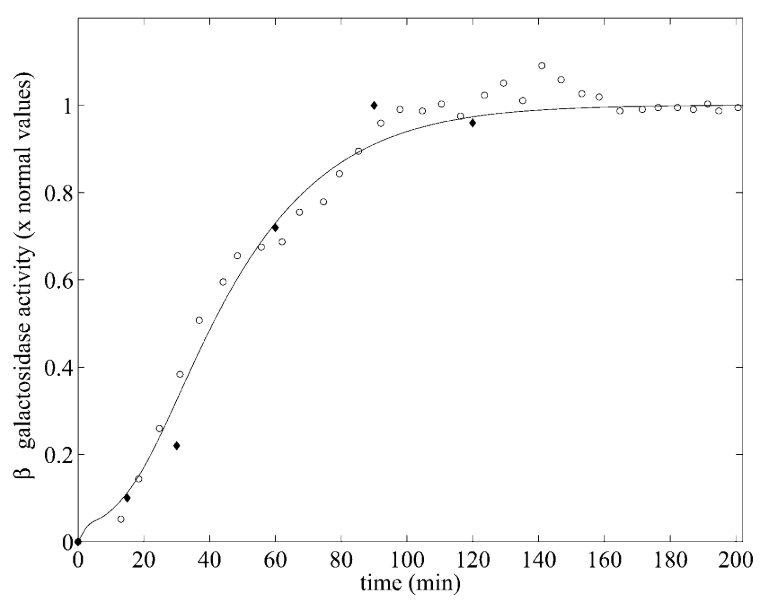
\includegraphics[width=1in]{Picture/lac-induces.png}
            %\caption{fig2}
            \end{minipage}%
            }%
    \caption{Comparism of ara and lac operon}
    \label{compare}
    \end{figure}
    We can observe a similar trend in both ara and lac operon model.The expression of their structure gene just increased.Therefore,i come up with this idea to subsitute ara with lac.
    
    But,there is one distinct difference between these two operons.
    The AraR is a \textbf{monomer} protein.There does not exist any interaction within it.We will make a further discussion afterwards.

    \section{Modeling of Lac promoter}
    
\end{document}